\chapter{Introduction to 5G and Key Technologies}
\label{chapter2}
The rapid advancement in the wireless communications shows the huge success in the wireless communication system. The advancement started with second generation (2G) system's debut in 1991 which were commercially launched on the GSM standard in Finland by Radiolinja. 2G systems were significantly more spectrally efficient compared to their predecessors and 2G also introduced the data services for mobile starting with SMS text messages, picture messages and multimedia messages (MMS). From 2G we migrated to 3G system which were first launched in 2001 and had fast mobile internet access. 3G also introduced video calls and mobile TV and was able to provide information transfer speed of at least 2 Mbit/s. The 4G wireless systems were designed to be fully based on IP telephony where all the voice communications and multimedia sessions are delivered over Internet protocol (IP) networks~\cite{4561570}. 4G systems use orthogonal frequency division multiplexing (OFDM), multiple-input multiple-output (MIMO), and link adaptation technologies for a long term evolution (LTE) radio interface. 4G wireless networks can support data rates of up to 1 Gb/s for low mobility and up to 100 Mb/s for high mobility scenarios. The next evolution in wireless mobile communications is the fifth generation (5G) which is expected to be deployed by 2020.

Due to a sharp increase in number of wireless mobile devices and the shortage of the wireless spectrum, researchers have started to investigate 5G wireless technologies. It is expected that the 5G network will achieve 1000 times the system capacity, 10 times the spectral efficiency, energy efficiency, data rate and 25 times the average cell throughput. This translates to a peak data rate of 10 Gb/s for low mobility and peak data rate of 1 Gb/s for high mobility scenarios. The table~\ref{tableG} below shows the comparison between 2G, 3G, 4G and 5G cellular communication system. 

\begin{table*}[!ht]
\centering
\label{tableG}
\caption{Cellular Technologies Comparison between different generations of deployed digital cellular networks. Data rates, standard and implementation technology is compared for the 3G, 4G and 5G}
\resizebox{\textwidth}{!}{\begin{tabular}{c c c}
\textbf{3G} & \textbf{4G} & \textbf{5G} \\\hline
1990/2002 & 2000/2010 & 2010/2022 \\\hline
2 Mbps & 200 Mbps -- 1 Gbps (low mobility) & 10 Gbps and higher (low mobility) \\\hline
WCDMA, CDMA-2000 & Unified Long Term Evolution (LTE) standard & In-progress \\\hline
\end{tabular}}
\end{table*}

\section{5G Cellular Architecture}
The base station density is increasing drastically due to the huge spike in the use of heterogeneous networks to support massive exchange of information over the air. The heterogeneous networks are already standardized in 4G but the architecture is not natively designed to support them. The huge network densification requires major changes in the cellular architecture of 5G communication system. Wireless users mostly stay indoors for about 80\% of the time, while only 20\% of the mobile users stay outdoors~\cite{4623708}. The conventional cellular architecture consists of an outdoor base station in the middle of a cell communicating with mobile users irrespective of the user's location. Since the signal incur a large penetration loss since it has through go through buildings, thus restricting the data rates, spectral and energy efficiency of the wireless transmissions. The key idea behind 5G cellular communication is to separate the outdoor and indoor scenarios so that the penetration loss and shadowing caused by buildings can be avoided. This will be achieved by using distributed antenna system (DAS) and massive MIMO technology (also referred to as ''Large-Scale Antenna Systems'') where spatially located antenna arrays with hundreds of antenna elements are deployed. Using large number of antenna arrays in base station renders the channels to the different devices quasi-orthogonal and very simple spatial multiplexing procedures quasi=optimal. The favourable action of the law of large numbers smoothens out frequency dependencies in the channel and thus leads to huge gains in the spectral efficiency~\cite{Boccardi2014}. The BSs deployed outdoors will be equipped with massive MIMO distributed around the cell and connected to the BS via optical fibers as a backbone network. The outdoor mobile users are normally equipped with very limited number of antenna elements, but
the devices can form a virtual massive MIMO links to increase the capacity and spectral efficiency. The Figure~\ref{5garch} shows the proposed heterogeneous 5G cellular architecture by C. Weng, et.al~\cite{Wang2014}. The proposed 5G cellular architecture consists of macrocells, microcells, small cells and relays. In this type of network, mobile users can be 
 
\begin{figure}[!ht]
	\centering
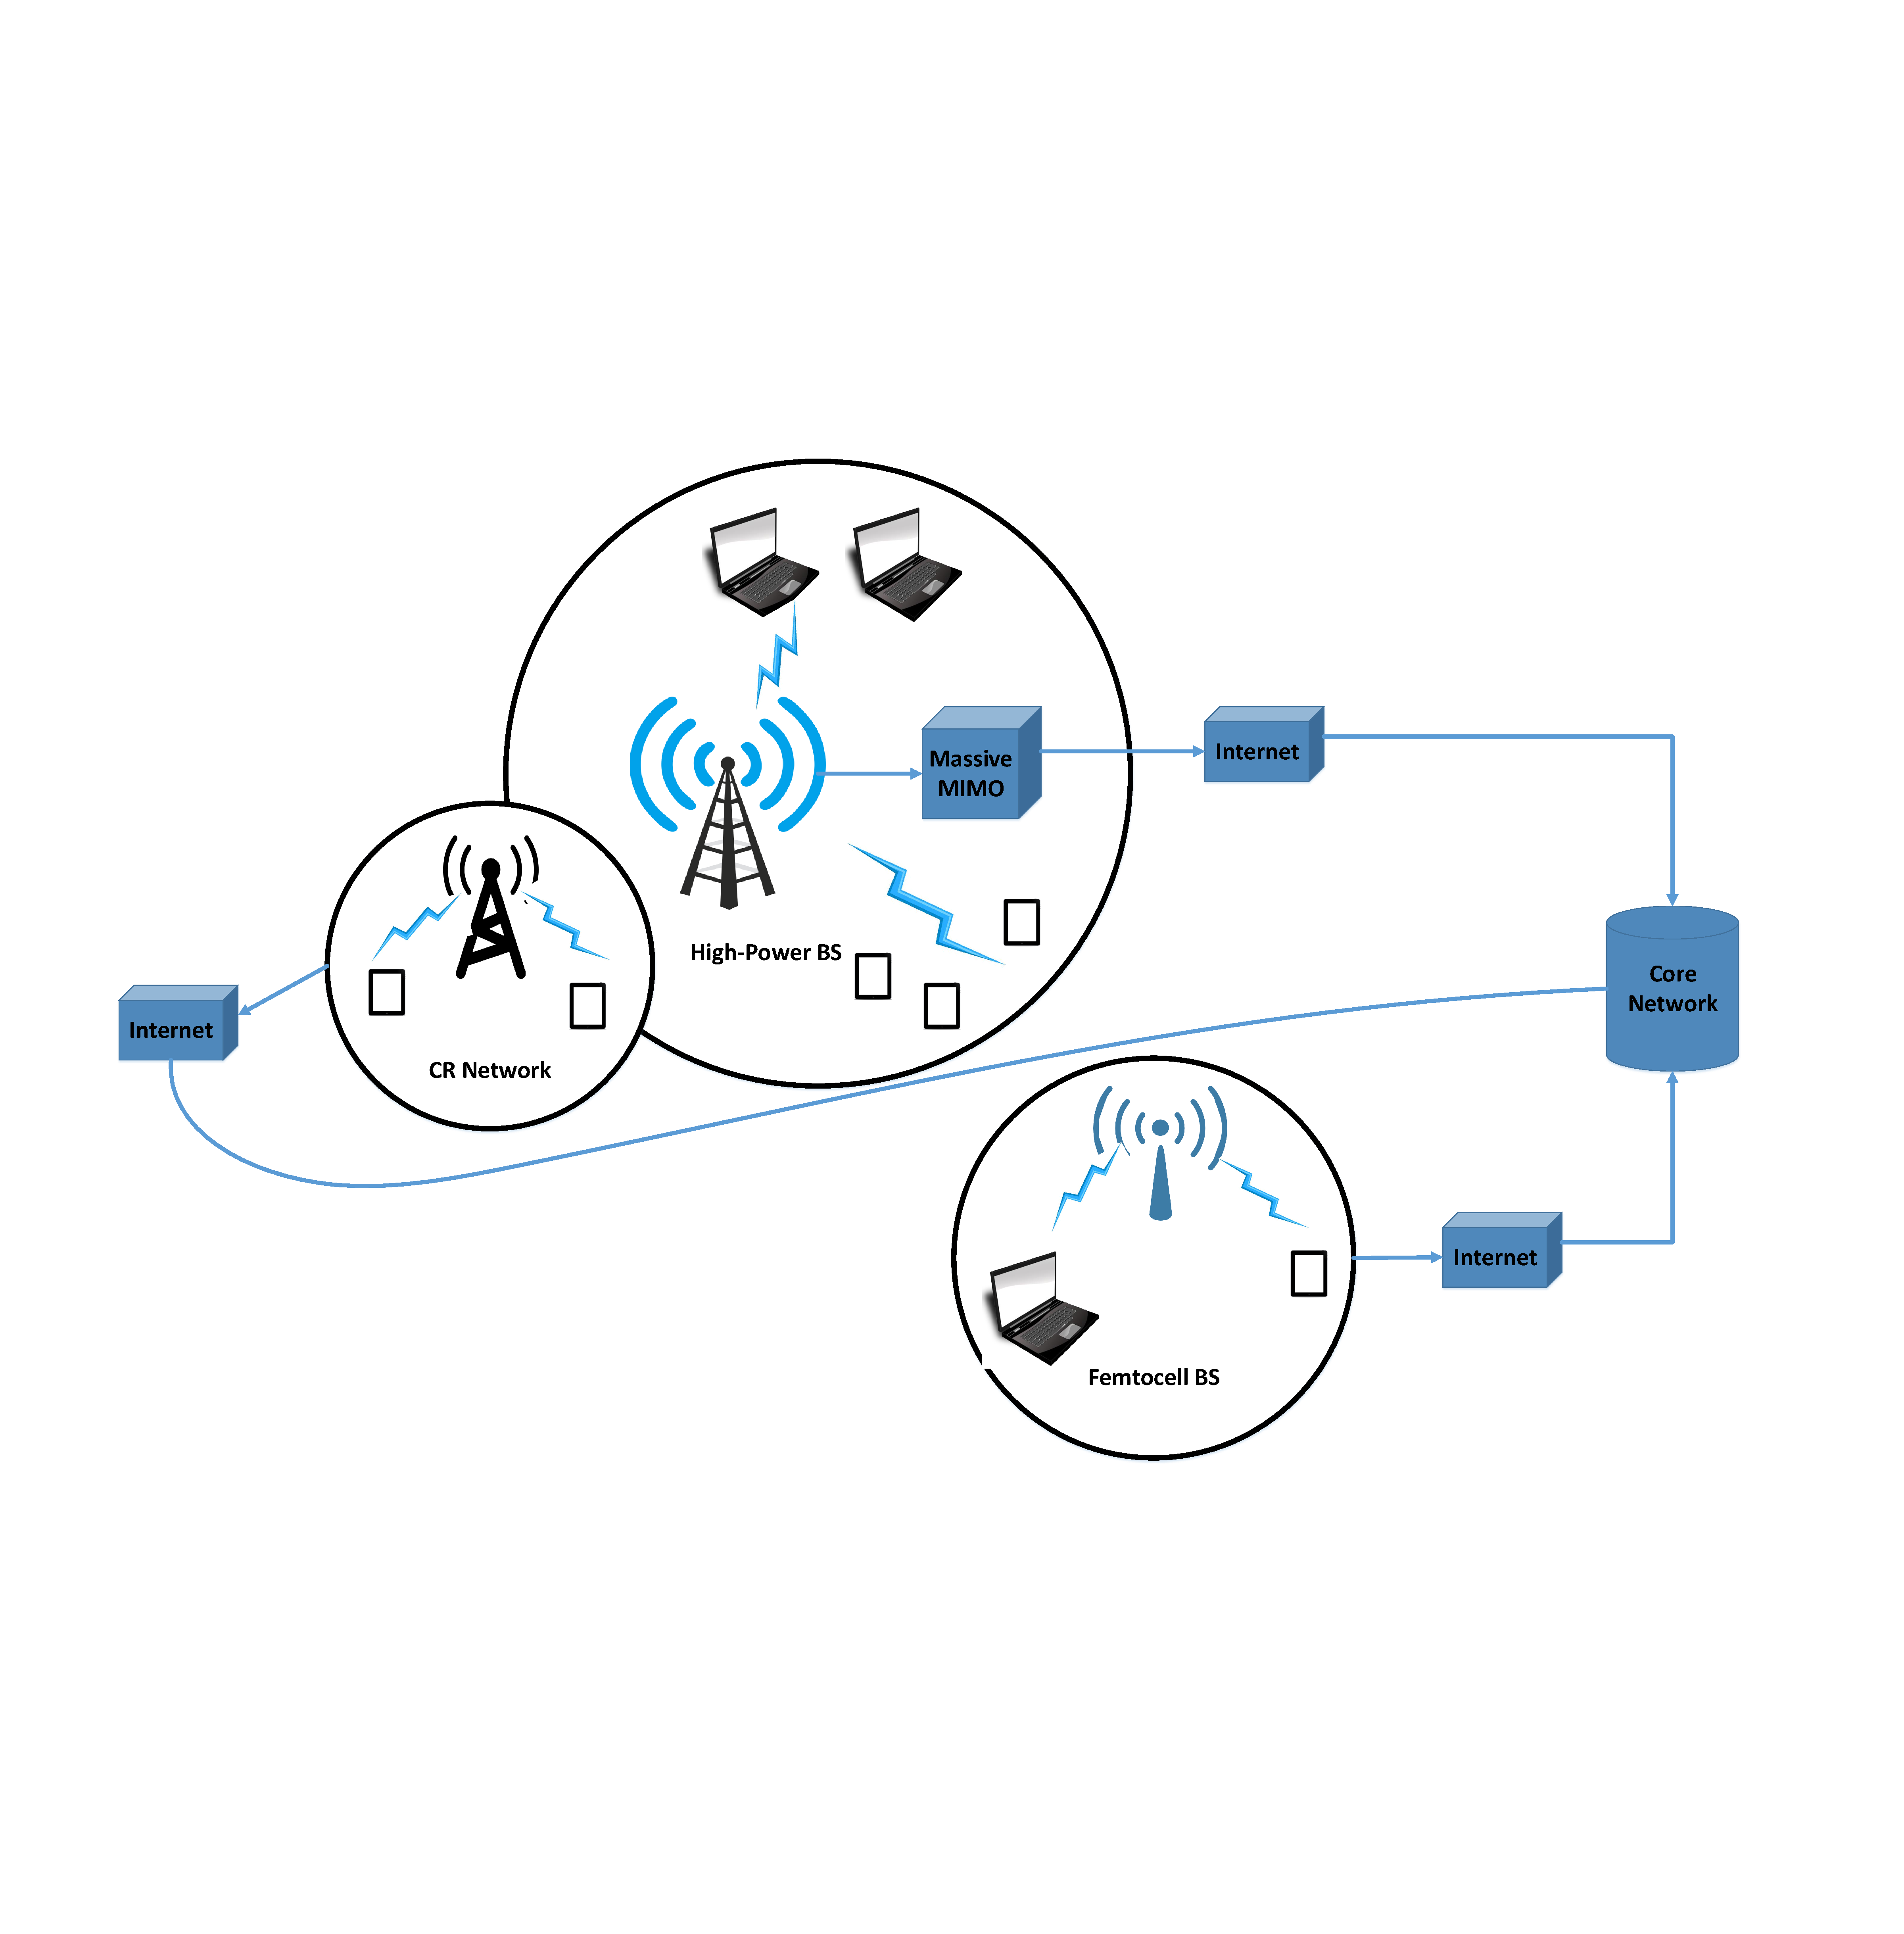
\includegraphics[width=\textwidth,height=10cm,keepaspectratio]{images/Gill/5G/5gsystemarch.eps}
	\caption{5G Architecture}
	\label{5garch}
\end{figure}

  

 
  
  Large antenna arrays will also be installed outside of every building to communicate with outdoor BSs or distributed antenna elements of BSs, possibly with line of sight (LoS) components. Large anten- na arrays have cables connected to the wireless access points inside the building communicating with indoor users. This will certainly increase the infrastructure cost in the short term while signifi- cantly improving the cell average throughput, spectral efficiency, energy efficiency, and data rate of the cellular system in the long run. Using such a cellular architecture, as indoor users only need to communicate with indoor wireless access points (not outdoor BSs) with large antenna arrays installed outside build- ings, many technologies can be utilized that are suitable for short-range communications with high data rates. Some examples include WiFi, femtocell, ultra wideband (UWB), mm-wave communications (3–300 GHz) [7], and visible light communications (VLC) (400–490 THz) [10]. It is worth mentioning that mm-wave and VLC technologies use higher frequencies not traditionally used for cellular communications. These high-frequency waves do not penetrate solid materials very well and can readily be absorbed or scattered by gases, rain, and foliage. Therefore, it is hard to use these waves for outdoor and long distance applications. However, with large bandwidths available, mm- wave and VLC technologies can greatly increase the transmission data rate for indoor scenarios. To solve the spectrum scarcity prob- lem, besides finding new spectrum not tradi- tionally used for wireless services (e.g., mm-wave communications and VLC), we can also try to improve the spectrum utilization of existing radio spectra, for example, via cogni- tive radio (CR) networks [11].
The 5G cellular architecture should also be a heterogeneous one, with macrocells, microcells, small cells, and relays. To accommodate high- mobility users such as users in vehicles and high- speed trains, we have proposed the mobile femtocell (MFemtocell) concept [12], which combines the concepts of mobile relay and fem- tocell. MFemtocells are located inside vehicles to communicate with users within the vehicle, while large antenna arrays are located outside the vehicle to communicate with outdoor BSs. An MFemtocell and its associated users are all viewed as a single unit to the BS. From the user point of view, an MFemtocell is seen as a regu- lar BS. This is very similar to the above idea of separating indoor (inside the vehicle) and out- door scenarios. It has been shown in [12] that users using MFemtocells can enjoy high-data-rate services with reduced signaling overhead. The above proposed 5G heterogeneous cellular architecture is illustrated in Fig. 1.







\section{Key Features of 5G System}
\subsection{Massive MIMO}
\subsection{Machine-to-Machine (M2M) Communication}
\subsection{Internet of Things (IoT)}

\section{5G using Millimeter Wave (mmWave)}

\section{5G in Vehicular Communication}

\section{Current Challenges}

\section{Summary}
This chapter outlined and examined the topics of jamming and anti-jamming techniques, and provided a foundation in communication system theory and advanced equalizer design.  Secondly it setup an understanding of Software-Defined Radio, the power of such an architecture, and examples of implementations and existing software for future designs.  Next, this thesis will consider a new anti-jamming technique and design an implementation of such a system.  After the implementation is investigated, the result of specific experiments on such an implementation will be analyzed.\\
